% Options for packages loaded elsewhere
\PassOptionsToPackage{unicode}{hyperref}
\PassOptionsToPackage{hyphens}{url}
%
\documentclass[
]{article}
\usepackage{lmodern}
\usepackage{amssymb,amsmath}
\usepackage{ifxetex,ifluatex}
\ifnum 0\ifxetex 1\fi\ifluatex 1\fi=0 % if pdftex
  \usepackage[T1]{fontenc}
  \usepackage[utf8]{inputenc}
  \usepackage{textcomp} % provide euro and other symbols
\else % if luatex or xetex
  \usepackage{unicode-math}
  \defaultfontfeatures{Scale=MatchLowercase}
  \defaultfontfeatures[\rmfamily]{Ligatures=TeX,Scale=1}
\fi
% Use upquote if available, for straight quotes in verbatim environments
\IfFileExists{upquote.sty}{\usepackage{upquote}}{}
\IfFileExists{microtype.sty}{% use microtype if available
  \usepackage[]{microtype}
  \UseMicrotypeSet[protrusion]{basicmath} % disable protrusion for tt fonts
}{}
\makeatletter
\@ifundefined{KOMAClassName}{% if non-KOMA class
  \IfFileExists{parskip.sty}{%
    \usepackage{parskip}
  }{% else
    \setlength{\parindent}{0pt}
    \setlength{\parskip}{6pt plus 2pt minus 1pt}}
}{% if KOMA class
  \KOMAoptions{parskip=half}}
\makeatother
\usepackage{xcolor}
\IfFileExists{xurl.sty}{\usepackage{xurl}}{} % add URL line breaks if available
\IfFileExists{bookmark.sty}{\usepackage{bookmark}}{\usepackage{hyperref}}
\hypersetup{
  pdftitle={NHL Goal Data},
  pdfauthor={null},
  hidelinks,
  pdfcreator={LaTeX via pandoc}}
\urlstyle{same} % disable monospaced font for URLs
\usepackage[margin=1in]{geometry}
\usepackage{color}
\usepackage{fancyvrb}
\newcommand{\VerbBar}{|}
\newcommand{\VERB}{\Verb[commandchars=\\\{\}]}
\DefineVerbatimEnvironment{Highlighting}{Verbatim}{commandchars=\\\{\}}
% Add ',fontsize=\small' for more characters per line
\usepackage{framed}
\definecolor{shadecolor}{RGB}{248,248,248}
\newenvironment{Shaded}{\begin{snugshade}}{\end{snugshade}}
\newcommand{\AlertTok}[1]{\textcolor[rgb]{0.94,0.16,0.16}{#1}}
\newcommand{\AnnotationTok}[1]{\textcolor[rgb]{0.56,0.35,0.01}{\textbf{\textit{#1}}}}
\newcommand{\AttributeTok}[1]{\textcolor[rgb]{0.77,0.63,0.00}{#1}}
\newcommand{\BaseNTok}[1]{\textcolor[rgb]{0.00,0.00,0.81}{#1}}
\newcommand{\BuiltInTok}[1]{#1}
\newcommand{\CharTok}[1]{\textcolor[rgb]{0.31,0.60,0.02}{#1}}
\newcommand{\CommentTok}[1]{\textcolor[rgb]{0.56,0.35,0.01}{\textit{#1}}}
\newcommand{\CommentVarTok}[1]{\textcolor[rgb]{0.56,0.35,0.01}{\textbf{\textit{#1}}}}
\newcommand{\ConstantTok}[1]{\textcolor[rgb]{0.00,0.00,0.00}{#1}}
\newcommand{\ControlFlowTok}[1]{\textcolor[rgb]{0.13,0.29,0.53}{\textbf{#1}}}
\newcommand{\DataTypeTok}[1]{\textcolor[rgb]{0.13,0.29,0.53}{#1}}
\newcommand{\DecValTok}[1]{\textcolor[rgb]{0.00,0.00,0.81}{#1}}
\newcommand{\DocumentationTok}[1]{\textcolor[rgb]{0.56,0.35,0.01}{\textbf{\textit{#1}}}}
\newcommand{\ErrorTok}[1]{\textcolor[rgb]{0.64,0.00,0.00}{\textbf{#1}}}
\newcommand{\ExtensionTok}[1]{#1}
\newcommand{\FloatTok}[1]{\textcolor[rgb]{0.00,0.00,0.81}{#1}}
\newcommand{\FunctionTok}[1]{\textcolor[rgb]{0.00,0.00,0.00}{#1}}
\newcommand{\ImportTok}[1]{#1}
\newcommand{\InformationTok}[1]{\textcolor[rgb]{0.56,0.35,0.01}{\textbf{\textit{#1}}}}
\newcommand{\KeywordTok}[1]{\textcolor[rgb]{0.13,0.29,0.53}{\textbf{#1}}}
\newcommand{\NormalTok}[1]{#1}
\newcommand{\OperatorTok}[1]{\textcolor[rgb]{0.81,0.36,0.00}{\textbf{#1}}}
\newcommand{\OtherTok}[1]{\textcolor[rgb]{0.56,0.35,0.01}{#1}}
\newcommand{\PreprocessorTok}[1]{\textcolor[rgb]{0.56,0.35,0.01}{\textit{#1}}}
\newcommand{\RegionMarkerTok}[1]{#1}
\newcommand{\SpecialCharTok}[1]{\textcolor[rgb]{0.00,0.00,0.00}{#1}}
\newcommand{\SpecialStringTok}[1]{\textcolor[rgb]{0.31,0.60,0.02}{#1}}
\newcommand{\StringTok}[1]{\textcolor[rgb]{0.31,0.60,0.02}{#1}}
\newcommand{\VariableTok}[1]{\textcolor[rgb]{0.00,0.00,0.00}{#1}}
\newcommand{\VerbatimStringTok}[1]{\textcolor[rgb]{0.31,0.60,0.02}{#1}}
\newcommand{\WarningTok}[1]{\textcolor[rgb]{0.56,0.35,0.01}{\textbf{\textit{#1}}}}
\usepackage{graphicx,grffile}
\makeatletter
\def\maxwidth{\ifdim\Gin@nat@width>\linewidth\linewidth\else\Gin@nat@width\fi}
\def\maxheight{\ifdim\Gin@nat@height>\textheight\textheight\else\Gin@nat@height\fi}
\makeatother
% Scale images if necessary, so that they will not overflow the page
% margins by default, and it is still possible to overwrite the defaults
% using explicit options in \includegraphics[width, height, ...]{}
\setkeys{Gin}{width=\maxwidth,height=\maxheight,keepaspectratio}
% Set default figure placement to htbp
\makeatletter
\def\fps@figure{htbp}
\makeatother
\setlength{\emergencystretch}{3em} % prevent overfull lines
\providecommand{\tightlist}{%
  \setlength{\itemsep}{0pt}\setlength{\parskip}{0pt}}
\setcounter{secnumdepth}{-\maxdimen} % remove section numbering

\title{NHL Goal Data}
\author{null}
\date{2020-12-10}

\begin{document}
\maketitle

\hypertarget{data}{%
\subsection{Data}\label{data}}

In this project I will be examining NHL goal data using the
game\_goals.csv dataset from HockeyReference.com (they put out the other
two datasets used in this post as well) that they put out after future
hall-of-famer Alexander Ovechkin scored his 700th career goal. The data
consists of 49384 observations of 25 variables. The variable season
represents each NHL season from 2006 to 2018.

The second dataset I will be using is the season\_goals.csv. The player
variable represents the individual players. The goals variable
represents the number of goals an individual scored in one season.

\begin{Shaded}
\begin{Highlighting}[]
\KeywordTok{library}\NormalTok{(tidyverse)}
\NormalTok{game_goals <-}\StringTok{ }\KeywordTok{read_csv}\NormalTok{(}\StringTok{"game_goals.csv"}\NormalTok{)}
\NormalTok{season_goals <-}\StringTok{ }\KeywordTok{read_csv}\NormalTok{(}\StringTok{"season_goals.csv"}\NormalTok{)}
\NormalTok{top_}\DecValTok{250}\NormalTok{_career <-}\StringTok{ }\KeywordTok{read_csv}\NormalTok{(}\StringTok{"top_250.csv"}\NormalTok{)}
\end{Highlighting}
\end{Shaded}

\hypertarget{question-1}{%
\subsection{Question 1}\label{question-1}}

Everyone who knows anything about hockey understands that Ovechkin is a
prolific goal scorer, but how does he measure up against the other great
goal scorers in NHL history?

\begin{Shaded}
\begin{Highlighting}[]
\CommentTok{# filter to only include seasons of >= 60 goals scored}
\NormalTok{GOAT_goal_scorers <-}\StringTok{ }\NormalTok{season_goals }\OperatorTok
\StringTok{  }\KeywordTok{filter}\NormalTok{(goals }\OperatorTok{>}\StringTok{ }\DecValTok{60}\NormalTok{)}
\end{Highlighting}
\end{Shaded}

I filtered out the data to only count seasons where a player scored 60
or more goals, because 1) there was too much data otherwise, and 2) it
gives a better sense of who had the most seasons with a
way-above-average number of goals scored.

\begin{Shaded}
\begin{Highlighting}[]
\KeywordTok{ggplot}\NormalTok{(GOAT_goal_scorers, }\DataTypeTok{mapping =} \KeywordTok{aes}\NormalTok{(player, goals, }\DataTypeTok{fill =}\NormalTok{ player)) }\OperatorTok{+}
\StringTok{  }\KeywordTok{geom_boxplot}\NormalTok{() }\OperatorTok{+}
\StringTok{  }\KeywordTok{theme}\NormalTok{(}\DataTypeTok{axis.text.x =} \KeywordTok{element_text}\NormalTok{(}\DataTypeTok{angle =} \DecValTok{-90}\NormalTok{, }\DataTypeTok{hjust =} \DecValTok{0}\NormalTok{)) }\OperatorTok{+}
\StringTok{  }\KeywordTok{theme}\NormalTok{(}\DataTypeTok{legend.position =} \StringTok{"None"}\NormalTok{) }\OperatorTok{+}
\StringTok{  }\CommentTok{# this is just so the color of the boxplots match the team, ore one of the teams, the player played for}
\StringTok{  }\KeywordTok{scale_fill_manual}\NormalTok{(}\DataTypeTok{values =} \KeywordTok{c}\NormalTok{(}\StringTok{"Alex Ovechkin"}\NormalTok{ =}\StringTok{ "red4"}\NormalTok{, }\StringTok{"Alexander Mogilny"}\NormalTok{ =}\StringTok{ "navy"}\NormalTok{, }\StringTok{"Bernie Nicholls"}\NormalTok{ =}\StringTok{ "gray4"}\NormalTok{, }\StringTok{"Bobby Hull"}\NormalTok{ =}\StringTok{ "red4"}\NormalTok{, }\StringTok{"Brett Hull"}\NormalTok{ =}\StringTok{ "green4"}\NormalTok{, }\StringTok{"Jari Kurri"}\NormalTok{ =}\StringTok{ "orangered"}\NormalTok{, }\StringTok{"Jaromir Jagr*"}\NormalTok{ =}\StringTok{ "yellow3"}\NormalTok{, }\StringTok{"Lanny McDonald"}\NormalTok{ =}\StringTok{ "red3"}\NormalTok{, }\StringTok{"Luc Robitaille"}\NormalTok{ =}\StringTok{ "darkorchid4"}\NormalTok{, }\StringTok{"Mario Lemieux"}\NormalTok{ =}\StringTok{ "yellow2"}\NormalTok{, }\StringTok{"Mike Bossy"}\NormalTok{ =}\StringTok{ "chocolate1"}\NormalTok{, }\StringTok{"Phil Esposito"}\NormalTok{ =}\StringTok{ "gold"}\NormalTok{, }\StringTok{"Reggie Leach"}\NormalTok{ =}\StringTok{ "darkorange"}\NormalTok{,  }\StringTok{"Steve Yzerman"}\NormalTok{ =}\StringTok{ "red3"}\NormalTok{, }\StringTok{"Teemu Selanne"}\NormalTok{ =}\StringTok{ "navyblue"}\NormalTok{, }\StringTok{"Wayne Gretzky"}\NormalTok{ =}\StringTok{ "mediumblue"}\NormalTok{))}
\end{Highlighting}
\end{Shaded}

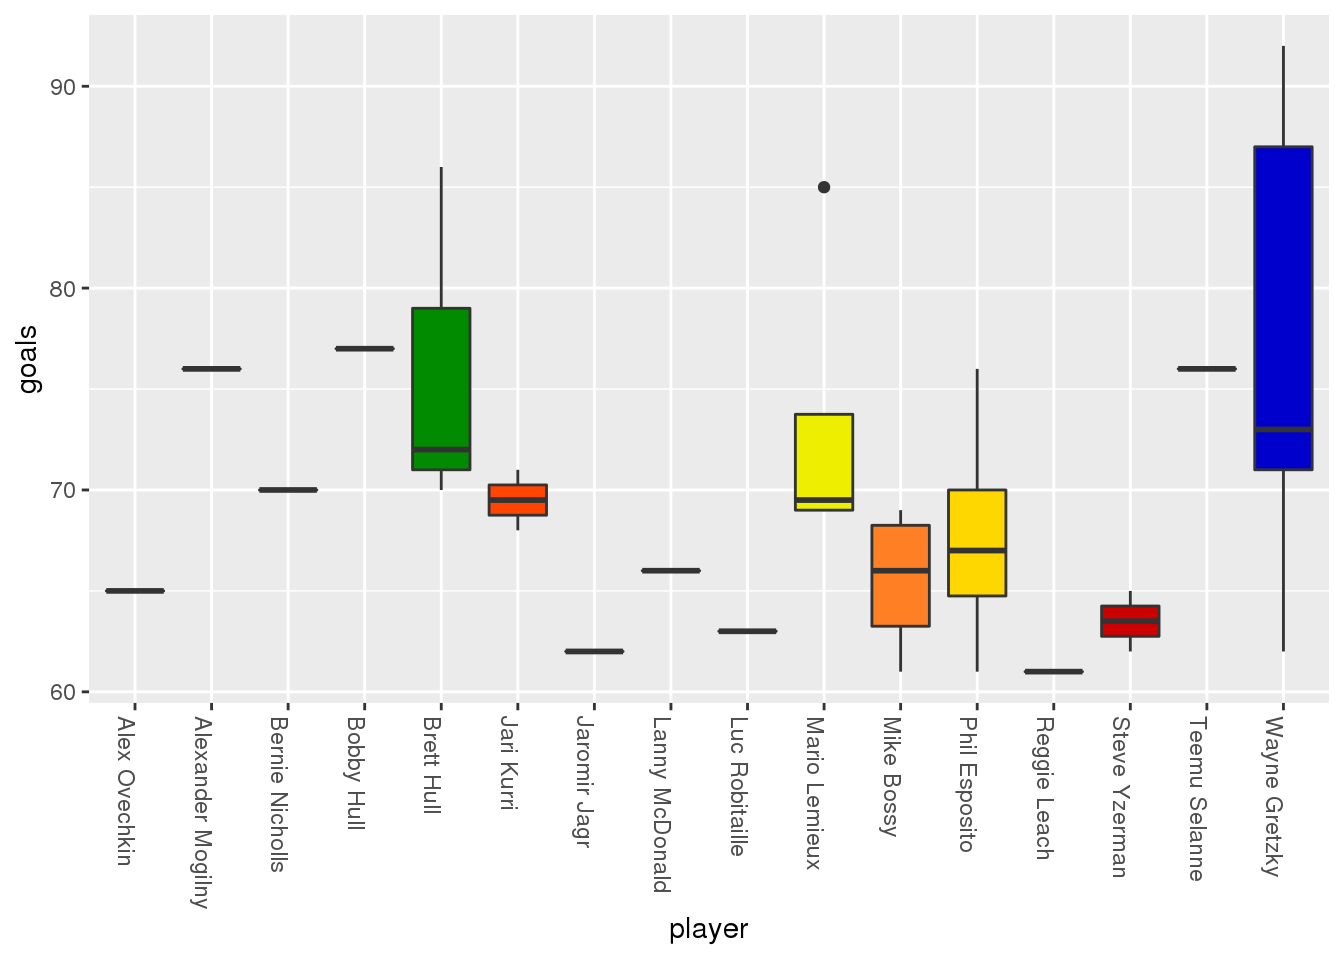
\includegraphics{index_files/figure-latex/unnamed-chunk-3-1.pdf}

This graphic gives an interesting insight into Ovechkin's place among
the all-time goal scoring greats in the history of the NHL. He has one
60+ goal season, which puts him in elite company. However, he still
isn't quite on the level of other all-time great goal scorers like Wayne
Gretzky, they call him ``The Great One'' for a reason, Brett Hull, and
``Super Mario'' Lemieux.

However, this graph is not the end all be all in determining the caliber
of goal scorer. Maurice ``Rocket'' Richard played for the Montreal
Canadiens from 1942-1960 and was an elite goal scorer, just look at his
then record 544 career goals upon retirement. He was so elite that the
Maurice ``Rocket'' Richard Trophy, also known as the Rocket Richard
Trophy, that is awarded annually to the leading goal scorer in the
National Hockey League is named after him. However, he played in the
Original Six era where they played 70 games a season compared to 80
games a season when Gretzky started out, and the 82 games played each
season in the modern day. Because of this Richard never scored 60+ goals
in one season, but that shouldn't automatically exclude him (and other
Original Six Era greats like Gordie Howe for that matter) from the
discussion of best goal scorers of all time.

\hypertarget{question-2}{%
\subsection{Question 2}\label{question-2}}

My next question that I want to investigate is how Ovechkin's path as a
prolific goal scorer in his career compares to the career trajectories
of the other greats that stood out in the previous graphic: Wayne
Gretzky, Mario Lemieux, and Brett Hull.

\begin{Shaded}
\begin{Highlighting}[]
\NormalTok{season_goals }\OperatorTok
\StringTok{  }\KeywordTok{filter}\NormalTok{(player }\OperatorTok{==}\StringTok{ "Alex Ovechkin"}\NormalTok{) }\OperatorTok
\StringTok{  }\KeywordTok{ggplot}\NormalTok{(season_goals, }\DataTypeTok{mapping =} \KeywordTok{aes}\NormalTok{(season, goals)) }\OperatorTok{+}
\StringTok{  }\KeywordTok{geom_point}\NormalTok{(}\DataTypeTok{shape=}\DecValTok{21}\NormalTok{, }\DataTypeTok{color =} \StringTok{"red"}\NormalTok{, }\DataTypeTok{fill =} \StringTok{"midnightblue"}\NormalTok{) }\OperatorTok{+}
\StringTok{  }\KeywordTok{geom_line}\NormalTok{(}\DataTypeTok{color=}\StringTok{"red"}\NormalTok{, }\DataTypeTok{group =} \DecValTok{1}\NormalTok{) }\OperatorTok{+}
\StringTok{  }\KeywordTok{theme}\NormalTok{(}\DataTypeTok{axis.text.x =} \KeywordTok{element_text}\NormalTok{(}\DataTypeTok{angle =} \DecValTok{-45}\NormalTok{, }\DataTypeTok{hjust =} \DecValTok{0}\NormalTok{)) }\OperatorTok{+}
\StringTok{  }\KeywordTok{ggtitle}\NormalTok{(}\StringTok{"Alex Ovechkin"}\NormalTok{) }\OperatorTok{+}
\StringTok{  }\KeywordTok{theme}\NormalTok{(}\DataTypeTok{plot.title =} \KeywordTok{element_text}\NormalTok{(}\DataTypeTok{hjust =} \FloatTok{0.5}\NormalTok{)) }\OperatorTok{+}
\StringTok{  }\KeywordTok{ylim}\NormalTok{(}\DecValTok{0}\NormalTok{, }\DecValTok{70}\NormalTok{)}
\end{Highlighting}
\end{Shaded}

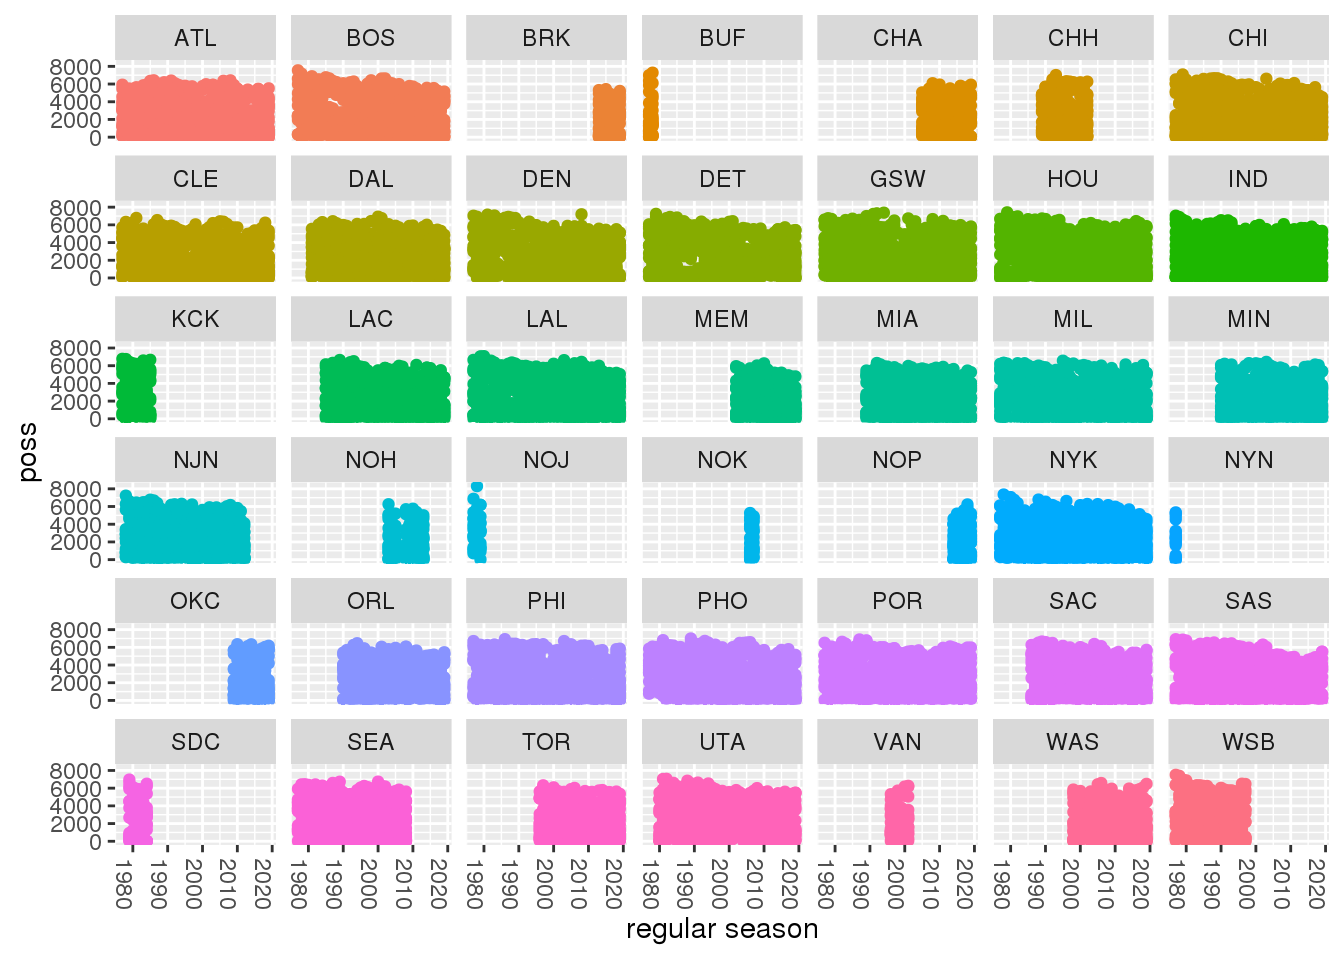
\includegraphics{index_files/figure-latex/unnamed-chunk-4-1.pdf}

\begin{Shaded}
\begin{Highlighting}[]
\NormalTok{season_goals }\OperatorTok
\StringTok{  }\KeywordTok{filter}\NormalTok{(player }\OperatorTok{==}\StringTok{ "Brett Hull"}\NormalTok{) }\OperatorTok
\StringTok{  }\KeywordTok{ggplot}\NormalTok{(season_goals, }\DataTypeTok{mapping =} \KeywordTok{aes}\NormalTok{(season, goals)) }\OperatorTok{+}
\StringTok{  }\KeywordTok{geom_point}\NormalTok{(}\DataTypeTok{shape=}\DecValTok{21}\NormalTok{, }\DataTypeTok{color =} \StringTok{"goldenrod1"}\NormalTok{, }\DataTypeTok{fill =} \StringTok{"forestgreen"}\NormalTok{) }\OperatorTok{+}
\StringTok{  }\KeywordTok{geom_line}\NormalTok{(}\DataTypeTok{color=}\StringTok{"forestgreen"}\NormalTok{, }\DataTypeTok{group =} \DecValTok{1}\NormalTok{) }\OperatorTok{+}
\StringTok{  }\KeywordTok{theme}\NormalTok{(}\DataTypeTok{axis.text.x =} \KeywordTok{element_text}\NormalTok{(}\DataTypeTok{angle =} \DecValTok{-45}\NormalTok{, }\DataTypeTok{hjust =} \DecValTok{0}\NormalTok{)) }\OperatorTok{+}
\StringTok{  }\KeywordTok{ggtitle}\NormalTok{(}\StringTok{"Brett Hull"}\NormalTok{) }\OperatorTok{+}
\StringTok{  }\KeywordTok{theme}\NormalTok{(}\DataTypeTok{plot.title =} \KeywordTok{element_text}\NormalTok{(}\DataTypeTok{hjust =} \FloatTok{0.5}\NormalTok{))}
\end{Highlighting}
\end{Shaded}

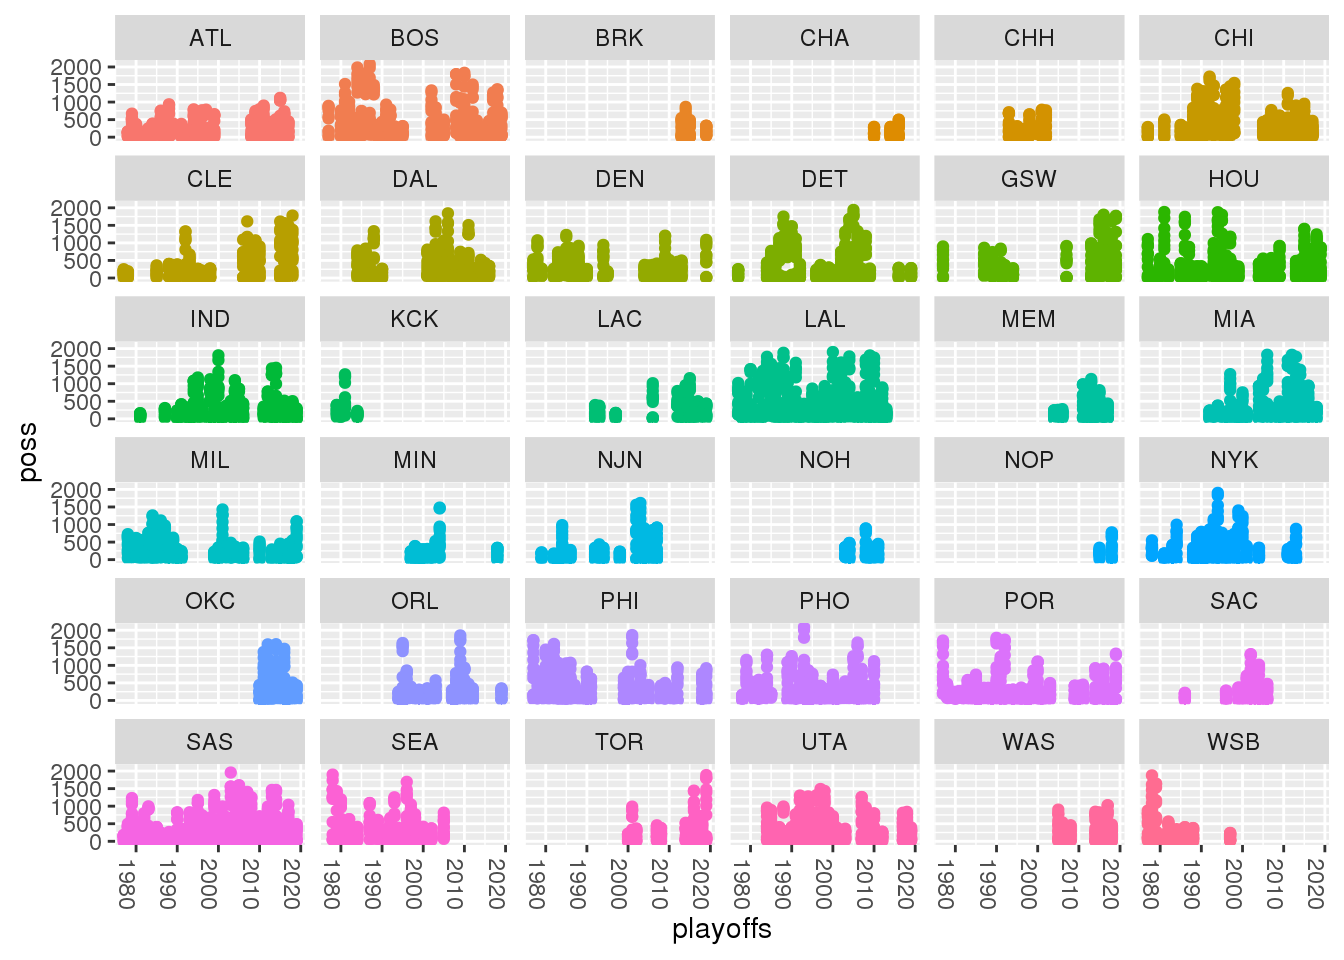
\includegraphics{index_files/figure-latex/unnamed-chunk-4-2.pdf}

\begin{Shaded}
\begin{Highlighting}[]
\NormalTok{season_goals }\OperatorTok
\StringTok{  }\KeywordTok{filter}\NormalTok{(player }\OperatorTok{==}\StringTok{ "Mario Lemieux"}\NormalTok{) }\OperatorTok
\StringTok{  }\KeywordTok{ggplot}\NormalTok{(season_goals, }\DataTypeTok{mapping =} \KeywordTok{aes}\NormalTok{(season, goals)) }\OperatorTok{+}
\StringTok{  }\KeywordTok{geom_point}\NormalTok{(}\DataTypeTok{shape=}\DecValTok{21}\NormalTok{, }\DataTypeTok{color =} \StringTok{"gray0"}\NormalTok{, }\DataTypeTok{fill =} \StringTok{"darkgoldenrod2"}\NormalTok{) }\OperatorTok{+}
\StringTok{  }\KeywordTok{geom_line}\NormalTok{(}\DataTypeTok{color=}\StringTok{"darkgoldenrod2"}\NormalTok{, }\DataTypeTok{group =} \DecValTok{1}\NormalTok{) }\OperatorTok{+}
\StringTok{  }\KeywordTok{theme}\NormalTok{(}\DataTypeTok{axis.text.x =} \KeywordTok{element_text}\NormalTok{(}\DataTypeTok{angle =} \DecValTok{-45}\NormalTok{, }\DataTypeTok{hjust =} \DecValTok{0}\NormalTok{)) }\OperatorTok{+}
\StringTok{  }\KeywordTok{ggtitle}\NormalTok{(}\StringTok{"Mario Lemieux"}\NormalTok{) }\OperatorTok{+}
\StringTok{  }\KeywordTok{theme}\NormalTok{(}\DataTypeTok{plot.title =} \KeywordTok{element_text}\NormalTok{(}\DataTypeTok{hjust =} \FloatTok{0.5}\NormalTok{))}
\end{Highlighting}
\end{Shaded}

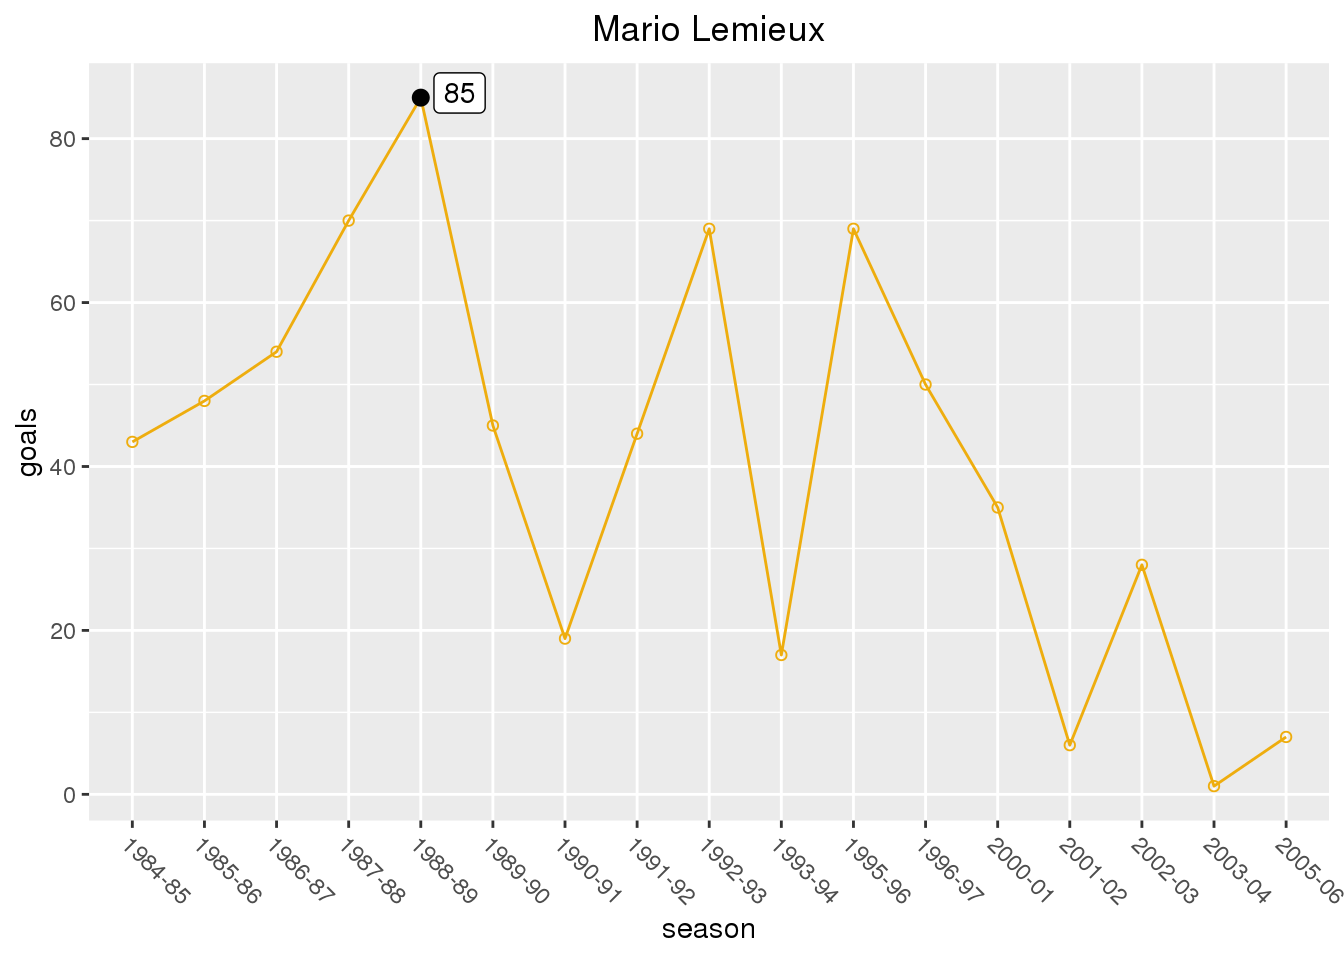
\includegraphics{index_files/figure-latex/unnamed-chunk-4-3.pdf}

\begin{Shaded}
\begin{Highlighting}[]
\NormalTok{season_goals }\OperatorTok
\StringTok{  }\KeywordTok{filter}\NormalTok{(player }\OperatorTok{==}\StringTok{ "Wayne Gretzky"}\NormalTok{) }\OperatorTok
\StringTok{  }\KeywordTok{ggplot}\NormalTok{(season_goals, }\DataTypeTok{mapping =} \KeywordTok{aes}\NormalTok{(season, goals)) }\OperatorTok{+}
\StringTok{  }\KeywordTok{geom_point}\NormalTok{(}\DataTypeTok{shape=}\DecValTok{21}\NormalTok{, }\DataTypeTok{color =} \StringTok{"darkorange"}\NormalTok{, }\DataTypeTok{fill =} \StringTok{"darkblue"}\NormalTok{) }\OperatorTok{+}
\StringTok{  }\KeywordTok{geom_line}\NormalTok{(}\DataTypeTok{color=}\StringTok{"darkblue"}\NormalTok{, }\DataTypeTok{group =} \DecValTok{1}\NormalTok{) }\OperatorTok{+}
\StringTok{  }\KeywordTok{theme}\NormalTok{(}\DataTypeTok{axis.text.x =} \KeywordTok{element_text}\NormalTok{(}\DataTypeTok{angle =} \DecValTok{-45}\NormalTok{, }\DataTypeTok{hjust =} \DecValTok{0}\NormalTok{)) }\OperatorTok{+}
\StringTok{  }\KeywordTok{ggtitle}\NormalTok{(}\StringTok{"Wayne Gretzky"}\NormalTok{) }\OperatorTok{+}
\StringTok{  }\KeywordTok{theme}\NormalTok{(}\DataTypeTok{plot.title =} \KeywordTok{element_text}\NormalTok{(}\DataTypeTok{hjust =} \FloatTok{0.5}\NormalTok{))}
\end{Highlighting}
\end{Shaded}

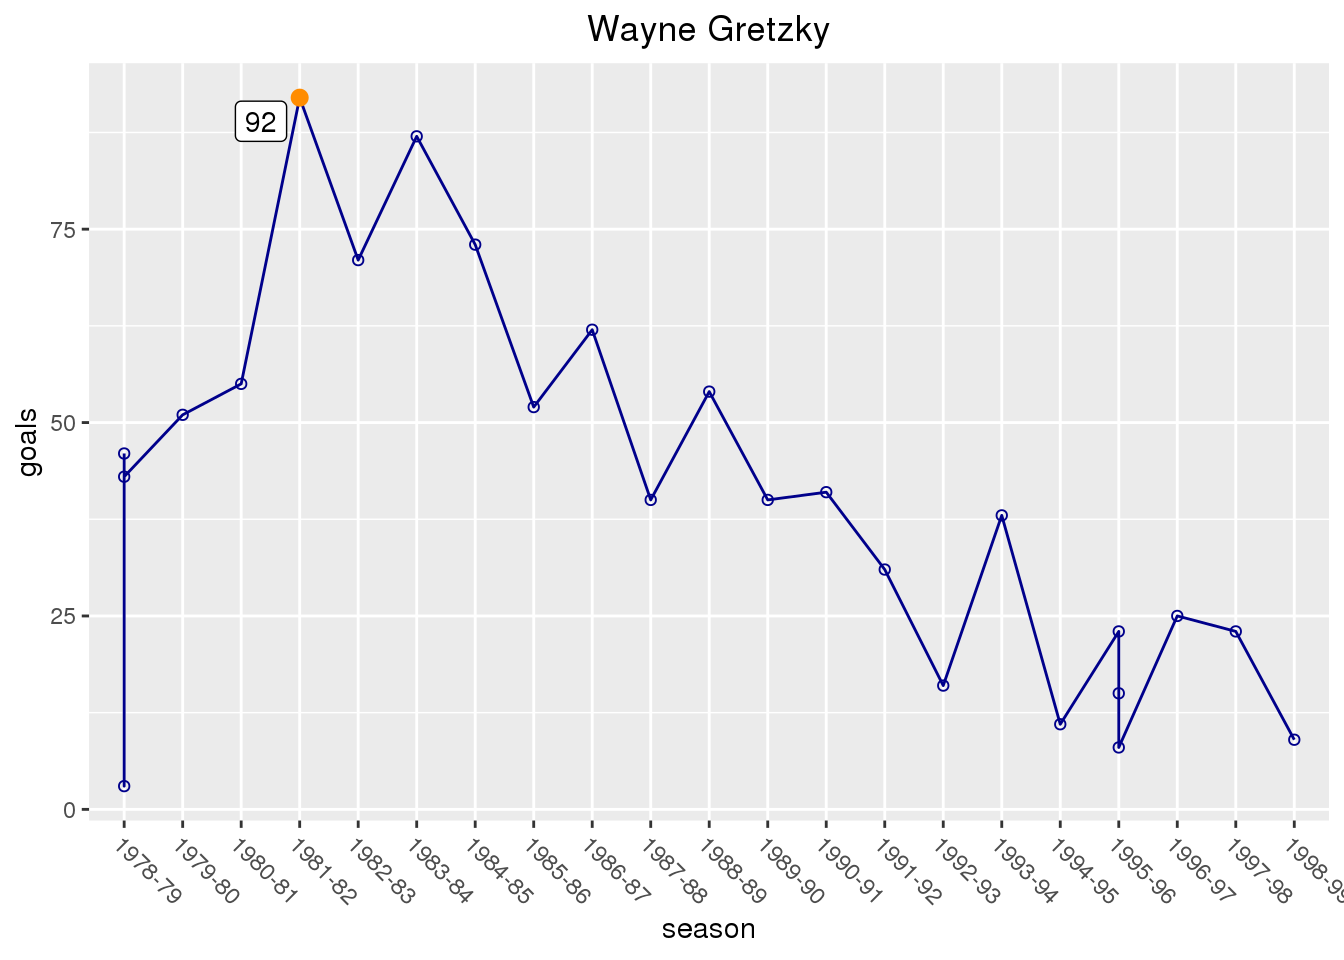
\includegraphics{index_files/figure-latex/unnamed-chunk-4-4.pdf}
\emph{For certain players there are years where there are 3 dots
representing total goals in a season instead of one. This is represents
a year in which the player was traded, so there is a dot representing
goals scored with each team, and a dot representing total goals. }Brett
Hull was traded from the Calgary Flames to the St.~Louis Blues in the
1987-1988 season. He scored 26 goals with Calgary, 6 goals with
St.~Louis, and 32 overall. *Wayne Gretzky was traded twice. While the
Edmonton Oilers were still in the WHA Gretzky was traded to them by the
Indianapolis Racers in the 1978-1979 season. He scored 3 goals with
Indianapolis, 43 goals with Edmonton, and 46 total. The second trade was
in the 1995-1996 season when the Los Angeles Kings traded him to the
St.~Louis Blues. He scored 15 goals with Los Angeles, 8 goals with
St.~Louis, and 23 goals total.

When comparing the data there is one factor that separates Ovechkin from
Hull, Lemieux, and Gretzky: Ovechkin is the only one that does not have
an 80 goal season. Since Ovechkin's strongest trait is goal scoring this
could be seen as something that might possibly hurt his reputation as
one of the best goal scorers. However, the outlook for Ovechkin may not
be as grim as that last statement might have made it seem. Super Mario's
85 goal season was a large outlier, and this can be seen on the boxplot
that represents his production in question 1 as well as in this graphic
since it shows he does not have another season of more than 70 goals.
Brett Hull's 86 goal season in 1990-1991 was not an outlier, but his
production steadily went down the rest of his career as he did not have
over 50 goals after his 7th season in 1993-1994. Gretzky had multiple
(he even had a 90 goal season) but, he is called ``The Great One'' for a
reason. But of the four players Ovechkin had the most instant impact
with 52 goals in his rookie season. This is the most for a rookie season
compared to the other three. Hull had 26, Lemieux had 43, and Gretzky
had 46. On top of this, Ovechkin has never had a season where he scored
under 30 goals whereas after their amazing seasons the other three
players regressed. Ovechkin doesn't have the best individual goal
scoring seasons of the four, but he is the most consistent.

\hypertarget{question-3}{%
\subsection{Question 3}\label{question-3}}

My final question is where does Ovechkin fall on the list of total
career goals, and whether or not it is possible for him to eventually
set the record for most career goals before he retires.

\begin{Shaded}
\begin{Highlighting}[]
\NormalTok{top_}\DecValTok{250}\NormalTok{_career }\OperatorTok
\StringTok{  }\KeywordTok{filter}\NormalTok{(total_goals }\OperatorTok{>}\StringTok{ }\DecValTok{675}\NormalTok{) }\OperatorTok
\StringTok{  }\KeywordTok{ggplot}\NormalTok{(top_}\DecValTok{250}\NormalTok{_career, }\DataTypeTok{mapping =} \KeywordTok{aes}\NormalTok{(raw_rank, total_goals)) }\OperatorTok{+}
\StringTok{  }\KeywordTok{geom_point}\NormalTok{(}\DataTypeTok{col =} \StringTok{"darkred"}\NormalTok{) }\OperatorTok{+}
\StringTok{  }\KeywordTok{gghighlight}\NormalTok{(raw_rank }\OperatorTok{>}\StringTok{ }\DecValTok{0} \OperatorTok{&}\StringTok{ }\NormalTok{raw_rank }\OperatorTok{<}\StringTok{ }\DecValTok{2}\NormalTok{ ,}
              \DataTypeTok{label_key =}\NormalTok{ player,}
              \DataTypeTok{unhighlighted_colour =} \KeywordTok{alpha}\NormalTok{(}\StringTok{"steelblue"}\NormalTok{, }\FloatTok{0.4}\NormalTok{)) }\OperatorTok{+}
\StringTok{  }\KeywordTok{geom_point}\NormalTok{(}\DataTypeTok{col =} \StringTok{"darkred"}\NormalTok{, }\DataTypeTok{size =} \FloatTok{2.5}\NormalTok{) }\OperatorTok{+}
\StringTok{  }\KeywordTok{scale_x_continuous}\NormalTok{(}\DataTypeTok{breaks =} \KeywordTok{round}\NormalTok{(}\KeywordTok{seq}\NormalTok{(}\KeywordTok{min}\NormalTok{(}\DecValTok{0}\NormalTok{), }\KeywordTok{max}\NormalTok{(}\DecValTok{14}\NormalTok{), }\DataTypeTok{by =} \DecValTok{1}\NormalTok{),}\DecValTok{1}\NormalTok{)) }\OperatorTok{+}
\StringTok{  }\KeywordTok{scale_y_continuous}\NormalTok{(}\DataTypeTok{breaks =} \KeywordTok{round}\NormalTok{(}\KeywordTok{seq}\NormalTok{(}\KeywordTok{min}\NormalTok{(}\DecValTok{0}\NormalTok{), }\KeywordTok{max}\NormalTok{(}\DecValTok{900}\NormalTok{), }\DataTypeTok{by =} \DecValTok{25}\NormalTok{),}\DecValTok{1}\NormalTok{)) }
\end{Highlighting}
\end{Shaded}

\begin{verbatim}
## Warning: The `unhighlighted_colour` argument of `gghighlight()` is deprecated as of gghighlight 0.2.0.
## Please use the `unhighlighted_params` argument instead.
## This warning is displayed once every 8 hours.
## Call `lifecycle::last_warnings()` to see where this warning was generated.
\end{verbatim}

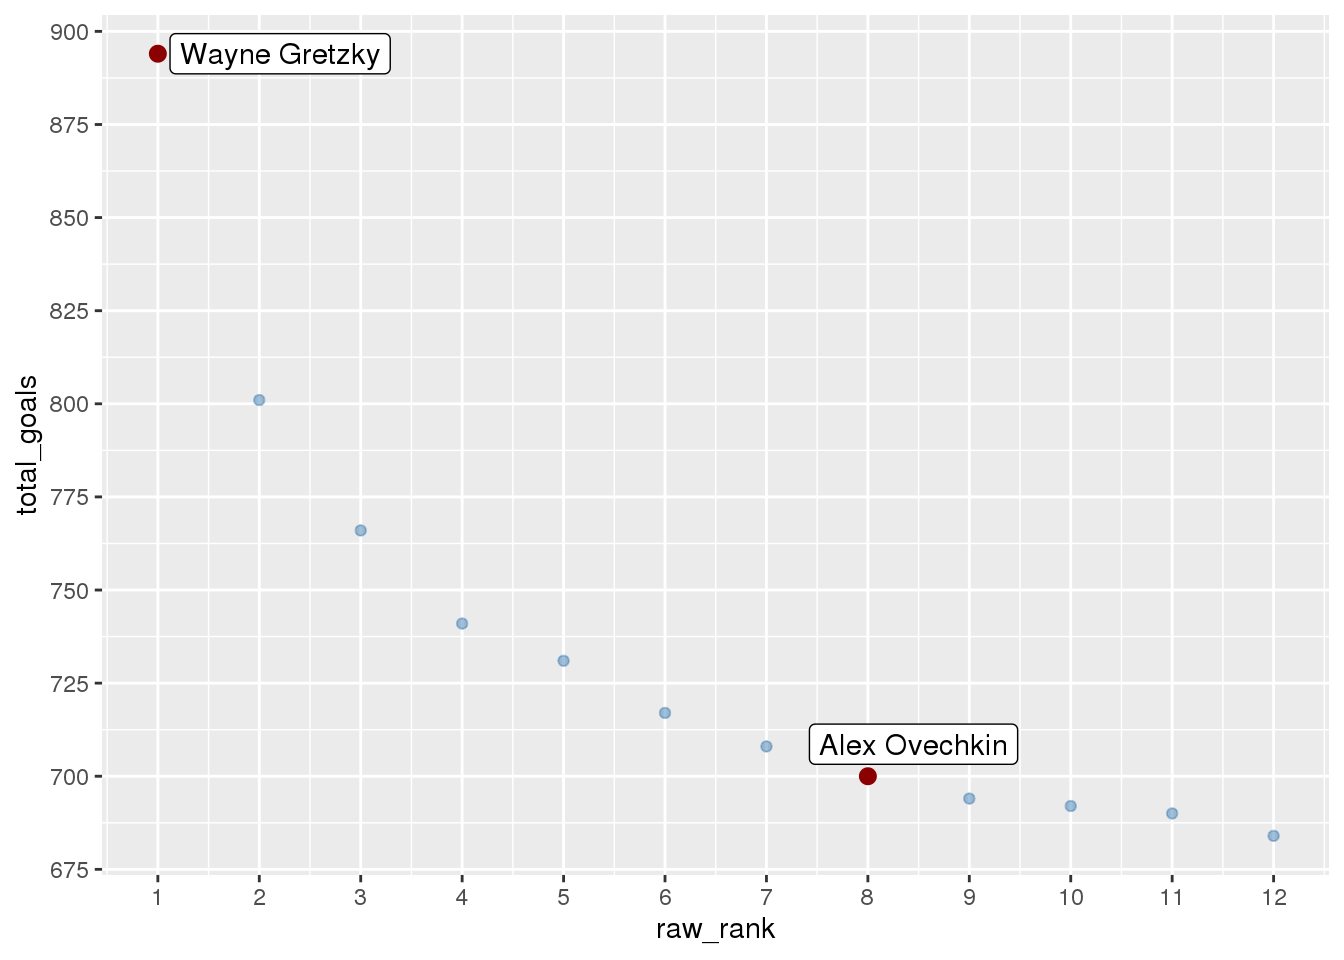
\includegraphics{index_files/figure-latex/unnamed-chunk-5-1.pdf}

\begin{Shaded}
\begin{Highlighting}[]
\NormalTok{top_}\DecValTok{250}\NormalTok{_career }\OperatorTok
\StringTok{  }\KeywordTok{filter}\NormalTok{(total_goals }\OperatorTok{>}\StringTok{ }\DecValTok{675}\NormalTok{) }\OperatorTok
\StringTok{  }\KeywordTok{ggplot}\NormalTok{(top_}\DecValTok{250}\NormalTok{_career, }\DataTypeTok{mapping =} \KeywordTok{aes}\NormalTok{(raw_rank, total_goals)) }\OperatorTok{+}
\StringTok{  }\KeywordTok{geom_point}\NormalTok{(}\DataTypeTok{col =} \StringTok{"darkred"}\NormalTok{) }\OperatorTok{+}
\StringTok{  }\KeywordTok{gghighlight}\NormalTok{(raw_rank }\OperatorTok{>}\StringTok{ }\DecValTok{7} \OperatorTok{&}\StringTok{ }\NormalTok{raw_rank }\OperatorTok{<}\StringTok{ }\DecValTok{9}\NormalTok{,}
              \DataTypeTok{label_key =}\NormalTok{ player,}
              \DataTypeTok{unhighlighted_colour =} \KeywordTok{alpha}\NormalTok{(}\StringTok{"steelblue"}\NormalTok{, }\FloatTok{0.4}\NormalTok{)) }\OperatorTok{+}
\StringTok{  }\KeywordTok{geom_point}\NormalTok{(}\DataTypeTok{col =} \StringTok{"darkred"}\NormalTok{, }\DataTypeTok{size =} \FloatTok{2.5}\NormalTok{) }\OperatorTok{+}
\StringTok{  }\KeywordTok{scale_x_continuous}\NormalTok{(}\DataTypeTok{breaks =} \KeywordTok{round}\NormalTok{(}\KeywordTok{seq}\NormalTok{(}\KeywordTok{min}\NormalTok{(}\DecValTok{0}\NormalTok{), }\KeywordTok{max}\NormalTok{(}\DecValTok{14}\NormalTok{), }\DataTypeTok{by =} \DecValTok{1}\NormalTok{),}\DecValTok{1}\NormalTok{)) }\OperatorTok{+}
\StringTok{  }\KeywordTok{scale_y_continuous}\NormalTok{(}\DataTypeTok{breaks =} \KeywordTok{round}\NormalTok{(}\KeywordTok{seq}\NormalTok{(}\KeywordTok{min}\NormalTok{(}\DecValTok{0}\NormalTok{), }\KeywordTok{max}\NormalTok{(}\DecValTok{900}\NormalTok{), }\DataTypeTok{by =} \DecValTok{25}\NormalTok{),}\DecValTok{1}\NormalTok{)) }
\end{Highlighting}
\end{Shaded}

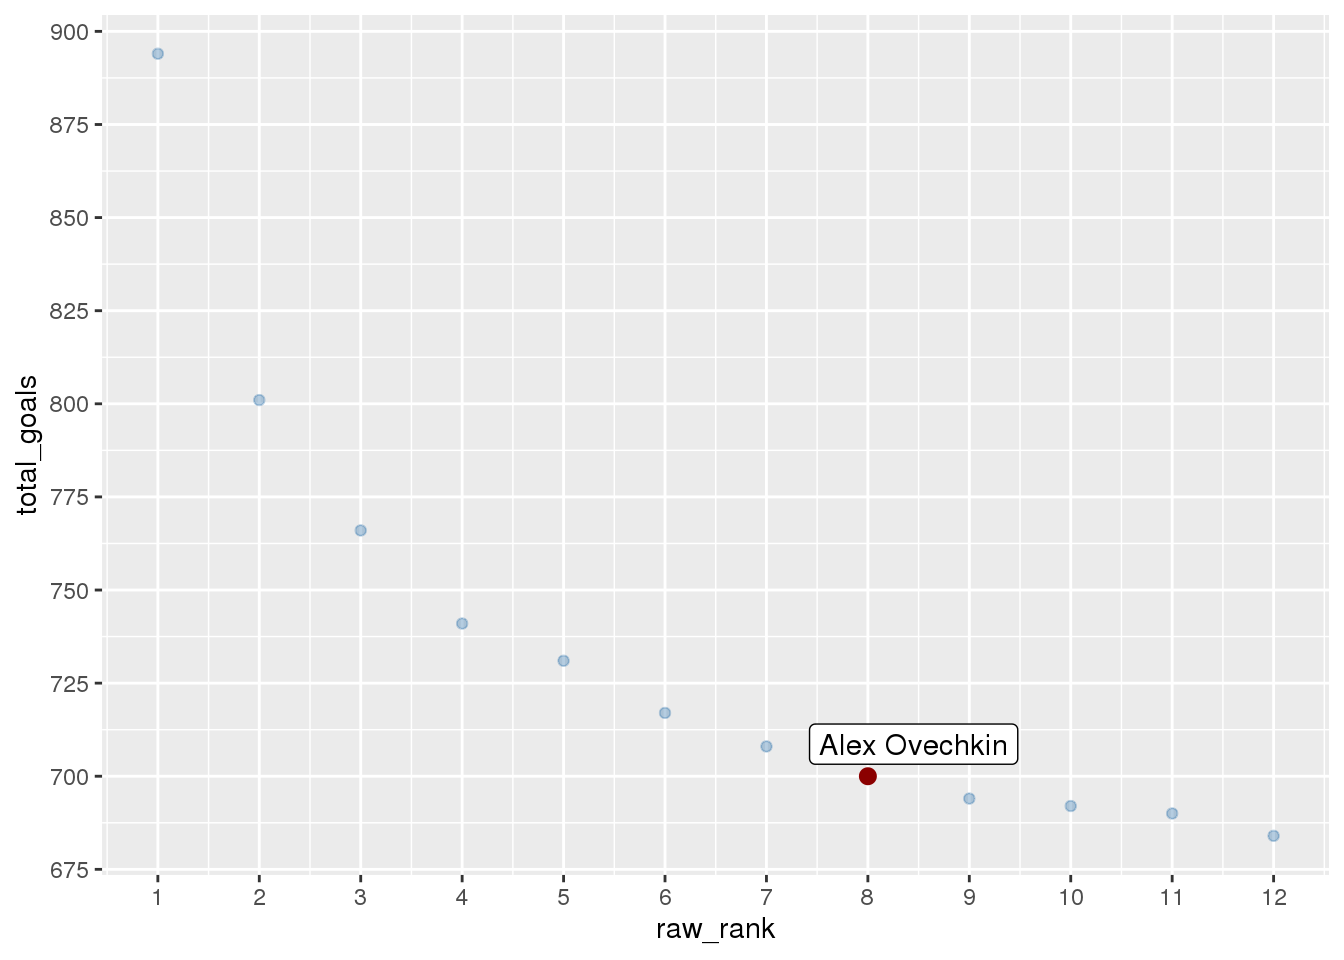
\includegraphics{index_files/figure-latex/unnamed-chunk-5-2.pdf}

These two graphics highlight Gretzky and Ovechkin on a list of top goal
scorers of all time. Gretzky is currently in 1st with 894 goals, and
Ovechkin is currently in 8th with 700 goals. Since the making of this
data set Ovechkin scored 6 more goals before the stoppage due to COVID
to reach a grand total of 706 career goals, which happens to put him 2
goals behind number 7 on the all time list Mike Gartner who had 708
career goals. Ovechkin has played in the NHL for 15 seasons. To get an
average of how many goals he scores per season we can divide his 706
career goals by his 15 seasons.

\begin{Shaded}
\begin{Highlighting}[]
\NormalTok{a <-}\StringTok{ }\DecValTok{706} \OperatorTok{/}\StringTok{ }\DecValTok{15}
\KeywordTok{print}\NormalTok{(a)}
\end{Highlighting}
\end{Shaded}

\begin{verbatim}
## [1] 47.06667
\end{verbatim}

Now, since Ovechkin has 186 less career goals than Gretzky we'll divide
that number by his career goals per season average to see how many
seasons of similar production it would take to catch Gretzky.

\begin{Shaded}
\begin{Highlighting}[]
\DecValTok{186} \OperatorTok{/}\StringTok{ }\NormalTok{a}
\end{Highlighting}
\end{Shaded}

\begin{verbatim}
## [1] 3.951841
\end{verbatim}

So this means it would take Ovechkin roughly 4 seasons of similar
production to catch Gretzky and have the most career goals of all time.
Ovechkin is 35 years old, so banking on him having averaging about 47
goals a season for the next 4 seasons might not be very realistic since
he is likely due for a decrease in production. However, Ovechkin is one
of the best ever at consistently scoring a lot of goals. He has the
second most 40-goal seasons of all time with 11, 1 less than Gretzky's
12. He also comes in second place all time for 50-goal seasons with 8,
Gretzky and Mike Bossy are tied for first with 9.

\hypertarget{conclusion}{%
\subsection{Conclusion}\label{conclusion}}

Ovechkin's career is not even over yet he is already in elite company
thanks to his goal scoring prowess. The purpose of this investigation
was to see if he would be able to one day have the title as the greatest
goal scorer of all time. The findings suggest that even though he is
likely due for a dip in production, surpassing Gretzky does not look
like an unattainable goal for Alexander Ovechkin.

However, does he have to surpass Gretzky to attain this title? Gretzky
has more goals, but he also played in an era where players simply scored
more than they do now. According to Steve Dongle of \emph{Sportsnet}, in
the 2016-2017 season NHL teams averaged 227 goals for and 227 against,
or about 5.5 goals per game. In the 1981-1982 season where Gretzky
scored an unthinkable 92 goals that number was over \textbf{8 goals per
game.} Because of cases like this \emph{hockey-reference.com} has
era-adjusted numbers for goals scored in a season to account for how
difficult, or not difficult, it was to score in the era the player
played in. Before this, Gordie Howe's 49 goals in the 1952-1953 season
would never have been brought up as one of the top goal scoring seasons
of all time. After adjusting for era his number of ``adjusted goals'' is
65 which is 11th all-time, which as a Red Wings fan makes me very happy.
The reason Mr.~Hockey's total went up so much can be chalked up to the
season being only 70 games long, and the goals per game being
\textbf{4.77.}

But what about Ovechkin's 65 goals in the 2007-2008 season? The number
of adjusted goals for Ovechkin in that season is \textbf{72}, second
only to Brett Hull's 78 that came from his 86 goal season in 1990-1991.
When looking at career records for adjusted goals scored Gordie Howe is
1st with 925, I mean he did play 35 seasons, Jagr is 2nd with 841, and
\textbf{Ovechkin is 3rd with 798}. This added wrinkle in the analysis of
Ovechkin's status among the goal scoring elite boosts his argument for
being one of the best. Not to mention what would have been his rookie
season in 2004-2005 was cancelled due to a lockout, the 2012-2013 was
shortened also due to a lockout, and the 2019-2020 season (in which he
was tied for the league lead in goals with 48) was cut short because of
COVID. His numbers likely be much higher if it wasn't for this. Had
these crazy incidents not happened Ovechkin would likely be much closer
to having the most career goals scored of all time, and that's without
adjusting for era. In conclusion, based off of analysis Ovechkin will be
the best goal scorer of all time by the time he retires- that is if he
isn't already.

\end{document}
